\PassOptionsToPackage{unicode=true}{hyperref} % options for packages loaded elsewhere
\PassOptionsToPackage{hyphens}{url}
\PassOptionsToPackage{dvipsnames,svgnames*,x11names*}{xcolor}
%
\documentclass[]{article}
\usepackage{lmodern}
\usepackage{amssymb,amsmath}
\usepackage{ifxetex,ifluatex}
\usepackage{fixltx2e} % provides \textsubscript
\ifnum 0\ifxetex 1\fi\ifluatex 1\fi=0 % if pdftex
  \usepackage[T1]{fontenc}
  \usepackage[utf8]{inputenc}
  \usepackage{textcomp} % provides euro and other symbols
\else % if luatex or xelatex
  \usepackage{unicode-math}
  \defaultfontfeatures{Ligatures=TeX,Scale=MatchLowercase}
\fi
% use upquote if available, for straight quotes in verbatim environments
\IfFileExists{upquote.sty}{\usepackage{upquote}}{}
% use microtype if available
\IfFileExists{microtype.sty}{%
\usepackage[]{microtype}
\UseMicrotypeSet[protrusion]{basicmath} % disable protrusion for tt fonts
}{}
\IfFileExists{parskip.sty}{%
\usepackage{parskip}
}{% else
\setlength{\parindent}{0pt}
\setlength{\parskip}{6pt plus 2pt minus 1pt}
}
\usepackage{xcolor}
\usepackage{hyperref}
\hypersetup{
            pdftitle={DPLYR Bisection--Evaluate Many Unknown Nonlinear Equations Jointly, Solve Roots for Strictly Monotonic Functions with Single Zero-Crossing},
            colorlinks=true,
            linkcolor=Maroon,
            citecolor=Blue,
            urlcolor=blue,
            breaklinks=true}
\urlstyle{same}  % don't use monospace font for urls
\usepackage[margin=1in]{geometry}
\usepackage{color}
\usepackage{fancyvrb}
\newcommand{\VerbBar}{|}
\newcommand{\VERB}{\Verb[commandchars=\\\{\}]}
\DefineVerbatimEnvironment{Highlighting}{Verbatim}{commandchars=\\\{\}}
% Add ',fontsize=\small' for more characters per line
\usepackage{framed}
\definecolor{shadecolor}{RGB}{248,248,248}
\newenvironment{Shaded}{\begin{snugshade}}{\end{snugshade}}
\newcommand{\AlertTok}[1]{\textcolor[rgb]{0.94,0.16,0.16}{#1}}
\newcommand{\AnnotationTok}[1]{\textcolor[rgb]{0.56,0.35,0.01}{\textbf{\textit{#1}}}}
\newcommand{\AttributeTok}[1]{\textcolor[rgb]{0.77,0.63,0.00}{#1}}
\newcommand{\BaseNTok}[1]{\textcolor[rgb]{0.00,0.00,0.81}{#1}}
\newcommand{\BuiltInTok}[1]{#1}
\newcommand{\CharTok}[1]{\textcolor[rgb]{0.31,0.60,0.02}{#1}}
\newcommand{\CommentTok}[1]{\textcolor[rgb]{0.56,0.35,0.01}{\textit{#1}}}
\newcommand{\CommentVarTok}[1]{\textcolor[rgb]{0.56,0.35,0.01}{\textbf{\textit{#1}}}}
\newcommand{\ConstantTok}[1]{\textcolor[rgb]{0.00,0.00,0.00}{#1}}
\newcommand{\ControlFlowTok}[1]{\textcolor[rgb]{0.13,0.29,0.53}{\textbf{#1}}}
\newcommand{\DataTypeTok}[1]{\textcolor[rgb]{0.13,0.29,0.53}{#1}}
\newcommand{\DecValTok}[1]{\textcolor[rgb]{0.00,0.00,0.81}{#1}}
\newcommand{\DocumentationTok}[1]{\textcolor[rgb]{0.56,0.35,0.01}{\textbf{\textit{#1}}}}
\newcommand{\ErrorTok}[1]{\textcolor[rgb]{0.64,0.00,0.00}{\textbf{#1}}}
\newcommand{\ExtensionTok}[1]{#1}
\newcommand{\FloatTok}[1]{\textcolor[rgb]{0.00,0.00,0.81}{#1}}
\newcommand{\FunctionTok}[1]{\textcolor[rgb]{0.00,0.00,0.00}{#1}}
\newcommand{\ImportTok}[1]{#1}
\newcommand{\InformationTok}[1]{\textcolor[rgb]{0.56,0.35,0.01}{\textbf{\textit{#1}}}}
\newcommand{\KeywordTok}[1]{\textcolor[rgb]{0.13,0.29,0.53}{\textbf{#1}}}
\newcommand{\NormalTok}[1]{#1}
\newcommand{\OperatorTok}[1]{\textcolor[rgb]{0.81,0.36,0.00}{\textbf{#1}}}
\newcommand{\OtherTok}[1]{\textcolor[rgb]{0.56,0.35,0.01}{#1}}
\newcommand{\PreprocessorTok}[1]{\textcolor[rgb]{0.56,0.35,0.01}{\textit{#1}}}
\newcommand{\RegionMarkerTok}[1]{#1}
\newcommand{\SpecialCharTok}[1]{\textcolor[rgb]{0.00,0.00,0.00}{#1}}
\newcommand{\SpecialStringTok}[1]{\textcolor[rgb]{0.31,0.60,0.02}{#1}}
\newcommand{\StringTok}[1]{\textcolor[rgb]{0.31,0.60,0.02}{#1}}
\newcommand{\VariableTok}[1]{\textcolor[rgb]{0.00,0.00,0.00}{#1}}
\newcommand{\VerbatimStringTok}[1]{\textcolor[rgb]{0.31,0.60,0.02}{#1}}
\newcommand{\WarningTok}[1]{\textcolor[rgb]{0.56,0.35,0.01}{\textbf{\textit{#1}}}}
\usepackage{graphicx,grffile}
\makeatletter
\def\maxwidth{\ifdim\Gin@nat@width>\linewidth\linewidth\else\Gin@nat@width\fi}
\def\maxheight{\ifdim\Gin@nat@height>\textheight\textheight\else\Gin@nat@height\fi}
\makeatother
% Scale images if necessary, so that they will not overflow the page
% margins by default, and it is still possible to overwrite the defaults
% using explicit options in \includegraphics[width, height, ...]{}
\setkeys{Gin}{width=\maxwidth,height=\maxheight,keepaspectratio}
\setlength{\emergencystretch}{3em}  % prevent overfull lines
\providecommand{\tightlist}{%
  \setlength{\itemsep}{0pt}\setlength{\parskip}{0pt}}
\setcounter{secnumdepth}{0}
% Redefines (sub)paragraphs to behave more like sections
\ifx\paragraph\undefined\else
\let\oldparagraph\paragraph
\renewcommand{\paragraph}[1]{\oldparagraph{#1}\mbox{}}
\fi
\ifx\subparagraph\undefined\else
\let\oldsubparagraph\subparagraph
\renewcommand{\subparagraph}[1]{\oldsubparagraph{#1}\mbox{}}
\fi

% set default figure placement to htbp
\makeatletter
\def\fps@figure{htbp}
\makeatother


\title{DPLYR Bisection--Evaluate Many Unknown Nonlinear Equations Jointly,
Solve Roots for Strictly Monotonic Functions with Single Zero-Crossing}
\author{}
\date{\vspace{-2.5em}}

\begin{document}
\maketitle

Go back to \href{http://fanwangecon.github.io/CodeDynaAsset/}{fan}'s
\href{https://fanwangecon.github.io/R4Econ/}{R4Econ} Repository or
\href{https://fanwangecon.github.io/Stat4Econ/}{Intro Stats with R}
Repository.

\hypertarget{issue-and-goal}{%
\section{Issue and Goal}\label{issue-and-goal}}

We want evaluate linear function
\(0=f(z_{ij}, x_i, y_i, \textbf{X}, \textbf{Y}, c, d)\). There are \(i\)
functions that have \(i\) specific \(x\) and \(y\). For each \(i\)
function, we evaluate along a grid of feasible values for \(z\), over
\(j\in J\) grid points, potentially looking for the \(j\) that is
closest to the root. \(\textbf{X}\) and \(\textbf{Y}\) are arrays common
across the \(i\) equations, and \(c\) and \(d\) are constants.

The evaluation strategy is the following, given min and max for \(z\)
that are specific for each \(j\), and given common number of grid
points, generate a matrix of \(z_{ij}\). Suppose there the number of
\(i\) is \(I\), and the number of grid points for \(j\) is \(J\).

\begin{enumerate}
\def\labelenumi{\arabic{enumi}.}
\tightlist
\item
  Generate a \(J \cdot I\) by \(3\) matrix where the columns are
  \(z,x,y\) as tibble
\item
  Follow
  \href{https://fanwangecon.github.io/R4Econ/support/function/fs_funceval.html}{this}
  Mutate to evaluate the \(f(\cdot)\) function.
\item
  Add two categorical columns for grid levels and wich \(i\), \(i\) and
  \(j\) index. Plot Mutate output evaluated column categorized by \(i\)
  as color and \(j\) as x-axis.
\end{enumerate}

\hypertarget{set-up}{%
\subsection{Set Up}\label{set-up}}

\begin{Shaded}
\begin{Highlighting}[]
\KeywordTok{rm}\NormalTok{(}\DataTypeTok{list =} \KeywordTok{ls}\NormalTok{(}\DataTypeTok{all.names =} \OtherTok{TRUE}\NormalTok{))}
\KeywordTok{options}\NormalTok{(}\DataTypeTok{knitr.duplicate.label =} \StringTok{'allow'}\NormalTok{)}
\end{Highlighting}
\end{Shaded}

\begin{Shaded}
\begin{Highlighting}[]
\KeywordTok{library}\NormalTok{(tidyverse)}
\KeywordTok{library}\NormalTok{(tidyr)}
\KeywordTok{library}\NormalTok{(knitr)}
\KeywordTok{library}\NormalTok{(kableExtra)}
\CommentTok{# file name}
\NormalTok{st_file_name =}\StringTok{ 'fs_func_graph_eval'}
\CommentTok{# Generate R File}
\KeywordTok{purl}\NormalTok{(}\KeywordTok{paste0}\NormalTok{(st_file_name, }\StringTok{".Rmd"}\NormalTok{), }\DataTypeTok{output=}\KeywordTok{paste0}\NormalTok{(st_file_name, }\StringTok{".R"}\NormalTok{), }\DataTypeTok{documentation =} \DecValTok{2}\NormalTok{)}
\CommentTok{# Generate PDF and HTML}
\CommentTok{# rmarkdown::render("C:/Users/fan/R4Econ/support/function/fs_funceval.Rmd", "pdf_document")}
\CommentTok{# rmarkdown::render("C:/Users/fan/R4Econ/support/function/fs_funceval.Rmd", "html_document")}
\end{Highlighting}
\end{Shaded}

\hypertarget{set-up-input-arrays}{%
\subsection{Set up Input Arrays}\label{set-up-input-arrays}}

There is a function that takes \(M=Q+P\) inputs, we want to evaluate
this function \(N\) times. Each time, there are \(M\) inputs, where all
but \(Q\) of the \(M\) inputs, meaning \(P\) of the \(M\) inputs, are
the same. In particular, \(P=Q*N\).

\[M = Q+P = Q + Q*N\]

Now we need to expand this by the number of choice grid. Each row,
representing one equation, is expanded by the number of choice grids. We
are graphically searching, or rather brute force searching, which means
if we have 100 individuals, we want to plot out the nonlinear equation
for each of these lines, and show graphically where each line crosses
zero. We achieve this, by evaluating the equation for each of the 100
individuals along a grid of feasible choices.

In this problem here, the feasible choices are shared across
individuals.

\begin{Shaded}
\begin{Highlighting}[]
\CommentTok{# Parameters}
\NormalTok{fl_rho =}\StringTok{ }\FloatTok{0.20}
\NormalTok{svr_id_var =}\StringTok{ 'INDI_ID'}

\CommentTok{# it_child_count = N, the number of children}
\NormalTok{it_N_child_cnt =}\StringTok{ }\DecValTok{4}
\CommentTok{# it_heter_param = Q, number of parameters that are heterogeneous across children}
\NormalTok{it_Q_hetpa_cnt =}\StringTok{ }\DecValTok{2}

\CommentTok{# P fixed parameters, nN is N dimensional, nP is P dimensional}
\NormalTok{ar_nN_A =}\StringTok{ }\KeywordTok{seq}\NormalTok{(}\OperatorTok{-}\DecValTok{2}\NormalTok{, }\DecValTok{2}\NormalTok{, }\DataTypeTok{length.out =}\NormalTok{ it_N_child_cnt)}
\NormalTok{ar_nN_alpha =}\StringTok{ }\KeywordTok{seq}\NormalTok{(}\FloatTok{0.1}\NormalTok{, }\FloatTok{0.9}\NormalTok{, }\DataTypeTok{length.out =}\NormalTok{ it_N_child_cnt)}
\NormalTok{ar_nP_A_alpha =}\StringTok{ }\KeywordTok{c}\NormalTok{(ar_nN_A, ar_nN_alpha)}

\CommentTok{# N by Q varying parameters}
\NormalTok{mt_nN_by_nQ_A_alpha =}\StringTok{ }\KeywordTok{cbind}\NormalTok{(ar_nN_A, ar_nN_alpha)}

\CommentTok{# Choice Grid for nutritional feasible choices for each}
\NormalTok{fl_N_agg =}\StringTok{ }\DecValTok{100}
\NormalTok{fl_N_min =}\StringTok{ }\DecValTok{0}
\NormalTok{it_N_choice_cnt_ttest =}\StringTok{ }\DecValTok{3}
\NormalTok{it_N_choice_cnt_dense =}\StringTok{ }\DecValTok{100}
\NormalTok{ar_N_choices_ttest =}\StringTok{ }\KeywordTok{seq}\NormalTok{(fl_N_min, fl_N_agg, }\DataTypeTok{length.out =}\NormalTok{ it_N_choice_cnt_ttest)}
\NormalTok{ar_N_choices_dense =}\StringTok{ }\KeywordTok{seq}\NormalTok{(fl_N_min, fl_N_agg, }\DataTypeTok{length.out =}\NormalTok{ it_N_choice_cnt_dense)}

\CommentTok{# Mesh Expand}
\NormalTok{tb_states_choices <-}\StringTok{ }\KeywordTok{as_tibble}\NormalTok{(mt_nN_by_nQ_A_alpha) }\OperatorTok\StringTok{ }\KeywordTok{rowid_to_column}\NormalTok{(}\DataTypeTok{var=}\NormalTok{svr_id_var) }
\NormalTok{tb_states_choices_ttest <-}\StringTok{ }\NormalTok{tb_states_choices }\OperatorTok\StringTok{ }\KeywordTok{expand_grid}\NormalTok{(}\DataTypeTok{choices =}\NormalTok{ ar_N_choices_ttest)}
\NormalTok{tb_states_choices_dense <-}\StringTok{ }\NormalTok{tb_states_choices }\OperatorTok\StringTok{ }\KeywordTok{expand_grid}\NormalTok{(}\DataTypeTok{choices =}\NormalTok{ ar_N_choices_dense)}

\CommentTok{# display}
\KeywordTok{summary}\NormalTok{(tb_states_choices_dense)}
\end{Highlighting}
\end{Shaded}

\begin{verbatim}
##     INDI_ID        ar_nN_A    ar_nN_alpha     choices   
##  Min.   :1.00   Min.   :-2   Min.   :0.1   Min.   :  0  
##  1st Qu.:1.75   1st Qu.:-1   1st Qu.:0.3   1st Qu.: 25  
##  Median :2.50   Median : 0   Median :0.5   Median : 50  
##  Mean   :2.50   Mean   : 0   Mean   :0.5   Mean   : 50  
##  3rd Qu.:3.25   3rd Qu.: 1   3rd Qu.:0.7   3rd Qu.: 75  
##  Max.   :4.00   Max.   : 2   Max.   :0.9   Max.   :100
\end{verbatim}

\begin{Shaded}
\begin{Highlighting}[]
\KeywordTok{kable}\NormalTok{(tb_states_choices_ttest) }\OperatorTok
\StringTok{  }\KeywordTok{kable_styling}\NormalTok{(}\DataTypeTok{bootstrap_options =} \KeywordTok{c}\NormalTok{(}\StringTok{"striped"}\NormalTok{, }\StringTok{"hover"}\NormalTok{, }\StringTok{"condensed"}\NormalTok{, }\StringTok{"responsive"}\NormalTok{))}
\end{Highlighting}
\end{Shaded}

INDI\_ID

ar\_nN\_A

ar\_nN\_alpha

choices

1

-2.0000000

0.1000000

0

1

-2.0000000

0.1000000

50

1

-2.0000000

0.1000000

100

2

-0.6666667

0.3666667

0

2

-0.6666667

0.3666667

50

2

-0.6666667

0.3666667

100

3

0.6666667

0.6333333

0

3

0.6666667

0.6333333

50

3

0.6666667

0.6333333

100

4

2.0000000

0.9000000

0

4

2.0000000

0.9000000

50

4

2.0000000

0.9000000

100

\hypertarget{apply-same-function-all-rows-some-inputs-row-specific-other-shared}{%
\section{Apply Same Function all Rows, Some Inputs Row-specific, other
Shared}\label{apply-same-function-all-rows-some-inputs-row-specific-other-shared}}

There are two types of inputs, row-specific inputs, and inputs that
should be applied for each row. The Function just requires all of these
inputs, it does not know what is row-specific and what is common for all
row. Dplyr recognizes which parameter inputs already existing in the
piped dataframe/tibble, given rowwise, those will be row-specific
inputs. Additional function parameters that do not exist in dataframe as
variable names, but that are pre-defined scalars or arrays will be
applied to all rows.

\begin{itemize}
\tightlist
\item
  @param string variable name of input where functions are evaluated,
  these are already contained in the dataframe, existing variable names,
  row specific, rowwise computation over these, each rowwise calculation
  using different rows: \emph{fl\_A}, \emph{fl\_alpha}, \emph{fl\_N}
\item
  @param scalar and array values that are applied to every rowwise
  calculation, all rowwise calculations using the same scalars and
  arrays:\emph{ar\_A}, \emph{ar\_alpha}, \emph{fl\_N\_agg},
  \emph{fl\_rho}
\item
  @param string output variable name
\end{itemize}

The function looks within group, finds min/max etc that are relevant.

\hypertarget{points-and-denser-dataframs-and-define-function}{%
\subsection{3 Points and Denser Dataframs and Define
Function}\label{points-and-denser-dataframs-and-define-function}}

\begin{Shaded}
\begin{Highlighting}[]
\CommentTok{# Convert Matrix to Tibble}
\NormalTok{ar_st_col_names =}\StringTok{ }\KeywordTok{c}\NormalTok{(svr_id_var,}\StringTok{'fl_A'}\NormalTok{, }\StringTok{'fl_alpha'}\NormalTok{)}
\NormalTok{tb_states_choices <-}\StringTok{ }\NormalTok{tb_states_choices }\OperatorTok\StringTok{ }\KeywordTok{rename_all}\NormalTok{(}\OperatorTok{~}\KeywordTok{c}\NormalTok{(ar_st_col_names))}
\NormalTok{ar_st_col_names =}\StringTok{ }\KeywordTok{c}\NormalTok{(svr_id_var,}\StringTok{'fl_A'}\NormalTok{, }\StringTok{'fl_alpha'}\NormalTok{, }\StringTok{'fl_N'}\NormalTok{)}
\NormalTok{tb_states_choices_ttest <-}\StringTok{ }\NormalTok{tb_states_choices_ttest }\OperatorTok\StringTok{ }\KeywordTok{rename_all}\NormalTok{(}\OperatorTok{~}\KeywordTok{c}\NormalTok{(ar_st_col_names))}
\NormalTok{tb_states_choices_dense <-}\StringTok{ }\NormalTok{tb_states_choices_dense }\OperatorTok\StringTok{ }\KeywordTok{rename_all}\NormalTok{(}\OperatorTok{~}\KeywordTok{c}\NormalTok{(ar_st_col_names))}

\CommentTok{# Define Implicit Function}
\NormalTok{ffi_nonlin_dplyrdo <-}\StringTok{ }\ControlFlowTok{function}\NormalTok{(fl_A, fl_alpha, fl_N, ar_A, ar_alpha, fl_N_agg, fl_rho)\{}
  \CommentTok{# scalar value that are row-specific, in dataframe already: *fl_A*, *fl_alpha*, *fl_N*}
  \CommentTok{# array and scalars not in dataframe, common all rows: *ar_A*, *ar_alpha*, *fl_N_agg*, *fl_rho*}

  \CommentTok{# Test Parameters}
  \CommentTok{# ar_A = ar_nN_A}
  \CommentTok{# ar_alpha = ar_nN_alpha}
  \CommentTok{# fl_N = 100}
  \CommentTok{# fl_rho = -1}
  \CommentTok{# fl_N_q = 10}

  \CommentTok{# Apply Function}
\NormalTok{  ar_p1_s1 =}\StringTok{ }\KeywordTok{exp}\NormalTok{((fl_A }\OperatorTok{-}\StringTok{ }\NormalTok{ar_A)}\OperatorTok{*}\NormalTok{fl_rho)}
\NormalTok{  ar_p1_s2 =}\StringTok{ }\NormalTok{(fl_alpha}\OperatorTok{/}\NormalTok{ar_alpha)}
\NormalTok{  ar_p1_s3 =}\StringTok{ }\NormalTok{(}\DecValTok{1}\OperatorTok{/}\NormalTok{(ar_alpha}\OperatorTok{*}\NormalTok{fl_rho }\OperatorTok{-}\StringTok{ }\DecValTok{1}\NormalTok{))}
\NormalTok{  ar_p1 =}\StringTok{ }\NormalTok{(ar_p1_s1}\OperatorTok{*}\NormalTok{ar_p1_s2)}\OperatorTok{^}\NormalTok{ar_p1_s3}
\NormalTok{  ar_p2 =}\StringTok{ }\NormalTok{fl_N}\OperatorTok{^}\NormalTok{((fl_alpha}\OperatorTok{*}\NormalTok{fl_rho}\DecValTok{-1}\NormalTok{)}\OperatorTok{/}\NormalTok{(ar_alpha}\OperatorTok{*}\NormalTok{fl_rho}\DecValTok{-1}\NormalTok{))}
\NormalTok{  ar_overall =}\StringTok{ }\NormalTok{ar_p1}\OperatorTok{*}\NormalTok{ar_p2}
\NormalTok{  fl_overall =}\StringTok{ }\NormalTok{fl_N_agg }\OperatorTok{-}\StringTok{ }\KeywordTok{sum}\NormalTok{(ar_overall)}

  \KeywordTok{return}\NormalTok{(fl_overall)}
\NormalTok{\}}
\end{Highlighting}
\end{Shaded}

\hypertarget{evaluate-at-three-choice-points-and-show-table}{%
\subsection{Evaluate at Three Choice Points and Show
Table}\label{evaluate-at-three-choice-points-and-show-table}}

In the example below, just show results evaluating over three choice
points and show table.

\begin{Shaded}
\begin{Highlighting}[]
\CommentTok{# fl_A, fl_alpha are from columns of tb_nN_by_nQ_A_alpha}
\NormalTok{tb_states_choices_ttest_eval =}\StringTok{ }\NormalTok{tb_states_choices_ttest }\OperatorTok\StringTok{ }\KeywordTok{rowwise}\NormalTok{() }\OperatorTok
\StringTok{                        }\KeywordTok{mutate}\NormalTok{(}\DataTypeTok{dplyr_eval =} \KeywordTok{ffi_nonlin_dplyrdo}\NormalTok{(fl_A, fl_alpha, fl_N,}
\NormalTok{                                                               ar_nN_A, ar_nN_alpha,}
\NormalTok{                                                               fl_N_agg, fl_rho))}
\CommentTok{# Show}
\KeywordTok{kable}\NormalTok{(tb_states_choices_ttest_eval) }\OperatorTok
\StringTok{  }\KeywordTok{kable_styling}\NormalTok{(}\DataTypeTok{bootstrap_options =} \KeywordTok{c}\NormalTok{(}\StringTok{"striped"}\NormalTok{, }\StringTok{"hover"}\NormalTok{, }\StringTok{"condensed"}\NormalTok{, }\StringTok{"responsive"}\NormalTok{))}
\end{Highlighting}
\end{Shaded}

INDI\_ID

fl\_A

fl\_alpha

fl\_N

dplyr\_eval

1

-2.0000000

0.1000000

0

100.00000

1

-2.0000000

0.1000000

50

-5666.95576

1

-2.0000000

0.1000000

100

-12880.28392

2

-0.6666667

0.3666667

0

100.00000

2

-0.6666667

0.3666667

50

-595.73454

2

-0.6666667

0.3666667

100

-1394.70698

3

0.6666667

0.6333333

0

100.00000

3

0.6666667

0.6333333

50

-106.51058

3

0.6666667

0.6333333

100

-323.94216

4

2.0000000

0.9000000

0

100.00000

4

2.0000000

0.9000000

50

22.55577

4

2.0000000

0.9000000

100

-51.97161

\hypertarget{evaluate-at-many-choice-points-and-show-graphically}{%
\subsection{Evaluate at Many Choice Points and Show
Graphically}\label{evaluate-at-many-choice-points-and-show-graphically}}

Same as above, but now we evaluate the function over the individuals at
many choice points so that we can graph things out.

\begin{Shaded}
\begin{Highlighting}[]
\CommentTok{# fl_A, fl_alpha are from columns of tb_nN_by_nQ_A_alpha}
\NormalTok{tb_states_choices_dense_eval =}\StringTok{ }\NormalTok{tb_states_choices_dense }\OperatorTok\StringTok{ }\KeywordTok{rowwise}\NormalTok{() }\OperatorTok
\StringTok{                        }\KeywordTok{mutate}\NormalTok{(}\DataTypeTok{dplyr_eval =} \KeywordTok{ffi_nonlin_dplyrdo}\NormalTok{(fl_A, fl_alpha, fl_N,}
\NormalTok{                                                               ar_nN_A, ar_nN_alpha,}
\NormalTok{                                                               fl_N_agg, fl_rho))}
\end{Highlighting}
\end{Shaded}

\begin{Shaded}
\begin{Highlighting}[]
\CommentTok{# Show}
\KeywordTok{dim}\NormalTok{(tb_states_choices_dense_eval)}
\end{Highlighting}
\end{Shaded}

\begin{verbatim}
## [1] 400   5
\end{verbatim}

\begin{Shaded}
\begin{Highlighting}[]
\KeywordTok{summary}\NormalTok{(tb_states_choices_dense_eval)}
\end{Highlighting}
\end{Shaded}

\begin{verbatim}
##     INDI_ID          fl_A       fl_alpha        fl_N       dplyr_eval       
##  Min.   :1.00   Min.   :-2   Min.   :0.1   Min.   :  0   Min.   :-12880.28  
##  1st Qu.:1.75   1st Qu.:-1   1st Qu.:0.3   1st Qu.: 25   1st Qu.: -1167.29  
##  Median :2.50   Median : 0   Median :0.5   Median : 50   Median :  -202.42  
##  Mean   :2.50   Mean   : 0   Mean   :0.5   Mean   : 50   Mean   : -1645.65  
##  3rd Qu.:3.25   3rd Qu.: 1   3rd Qu.:0.7   3rd Qu.: 75   3rd Qu.:     0.96  
##  Max.   :4.00   Max.   : 2   Max.   :0.9   Max.   :100   Max.   :   100.00
\end{verbatim}

\begin{Shaded}
\begin{Highlighting}[]
\NormalTok{lineplot <-}\StringTok{ }\NormalTok{tb_states_choices_dense_eval }\OperatorTok\StringTok{ }
\StringTok{    }\KeywordTok{ggplot}\NormalTok{(}\KeywordTok{aes}\NormalTok{(}\DataTypeTok{x=}\NormalTok{fl_N, }\DataTypeTok{y=}\NormalTok{dplyr_eval)) }\OperatorTok{+}
\StringTok{        }\KeywordTok{geom_line}\NormalTok{() }\OperatorTok{+}
\StringTok{        }\KeywordTok{facet_wrap}\NormalTok{( . }\OperatorTok{~}\StringTok{ }\NormalTok{INDI_ID, }\DataTypeTok{scales =} \StringTok{"free"}\NormalTok{) }\OperatorTok{+}\StringTok{ }
\StringTok{        }\KeywordTok{geom_hline}\NormalTok{(}\DataTypeTok{yintercept=}\DecValTok{0}\NormalTok{, }\DataTypeTok{linetype=}\StringTok{"dashed"}\NormalTok{, }
                \DataTypeTok{color =} \StringTok{"red"}\NormalTok{, }\DataTypeTok{size=}\DecValTok{1}\NormalTok{)}
        \KeywordTok{labs}\NormalTok{(}\DataTypeTok{title =} \StringTok{'Evaluate Non-Linear Functions to Search for Roots'}\NormalTok{,}
             \DataTypeTok{x =} \StringTok{'X values'}\NormalTok{,}
             \DataTypeTok{y =} \StringTok{'f(x)'}\NormalTok{,}
             \DataTypeTok{caption =} \StringTok{'Evaluating the Function'}\NormalTok{) }
\end{Highlighting}
\end{Shaded}

\begin{verbatim}
## $x
## [1] "X values"
## 
## $y
## [1] "f(x)"
## 
## $title
## [1] "Evaluate Non-Linear Functions to Search for Roots"
## 
## $caption
## [1] "Evaluating the Function"
## 
## attr(,"class")
## [1] "labels"
\end{verbatim}

\begin{Shaded}
\begin{Highlighting}[]
\KeywordTok{print}\NormalTok{(lineplot)}
\end{Highlighting}
\end{Shaded}

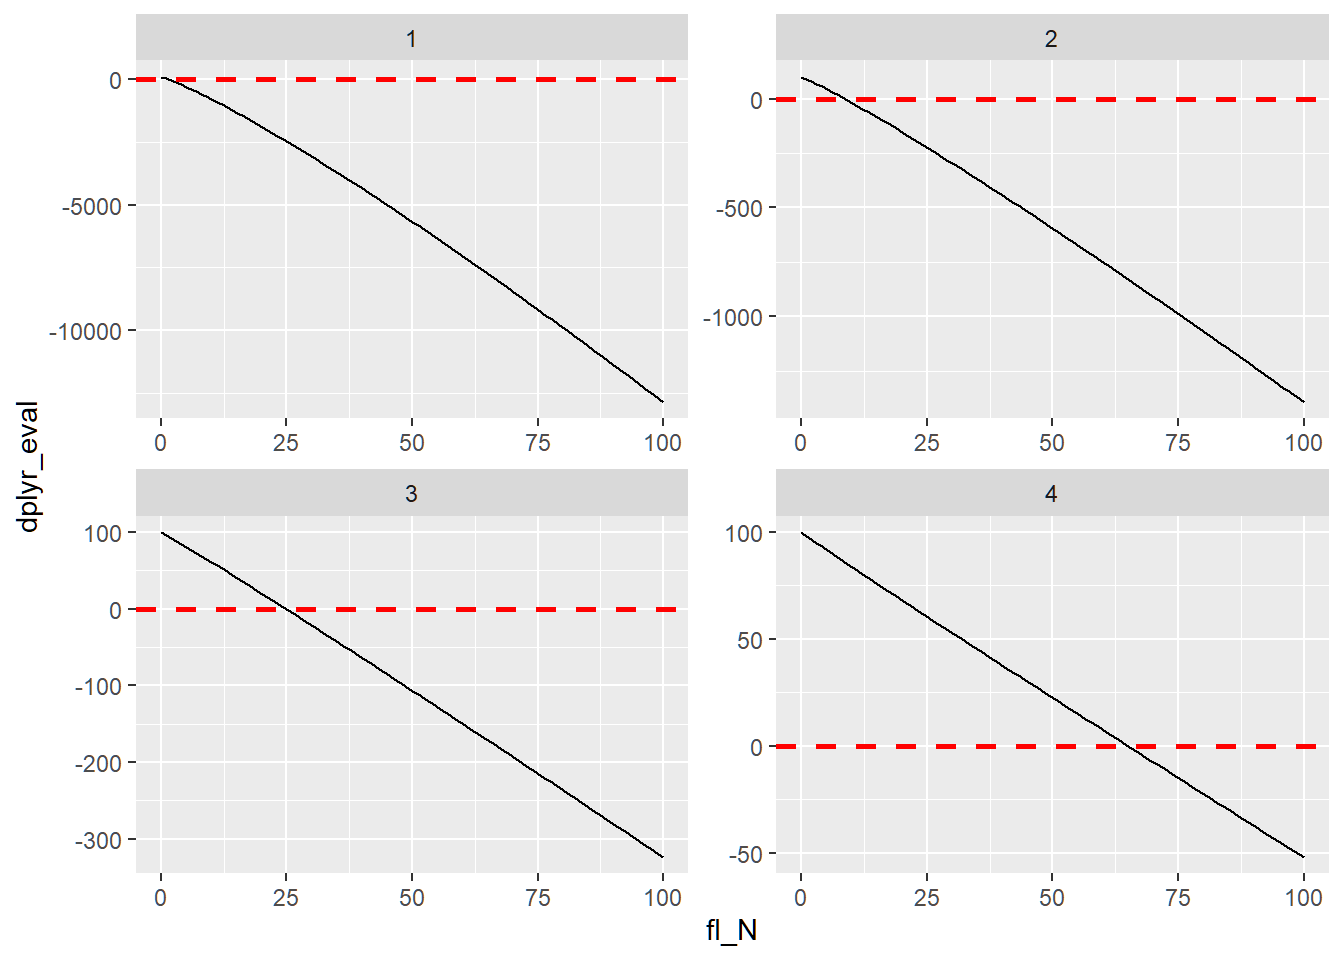
\includegraphics{fs_func_graph_eval_files/figure-latex/graph many evaluations-1.pdf}

\hypertarget{bisection-solve-optimal-choice-for-each-individual}{%
\section{Bisection Solve Optimal Choice for Each
Individual}\label{bisection-solve-optimal-choice-for-each-individual}}

The bisection specific code does not need to do much.

\begin{itemize}
\tightlist
\item
  @param list variables in file for grouping, each group is an
  individual for whom we want to calculate optimal choice for using
  bisection.
\item
  @param string variable name of input where functions are evaluated,
  these are already contained in the dataframe, existing variable names,
  row specific, rowwise computation over these, each rowwise calculation
  using different rows.
\item
  @param scalar and array values that are applied to every rowwise
  calculation, all rowwise calculations using the same scalars and
  arrays.
\item
  @param string output variable name
\end{itemize}

\hypertarget{bisection-algorithm}{%
\subsection{Bisection Algorithm}\label{bisection-algorithm}}

This is how I implement the bisection algorithm, when we know the
bounding minimum and maximum to be below and above zero already.

\begin{enumerate}
\def\labelenumi{\arabic{enumi}.}
\tightlist
\item
  Evaluate \(f^0_a = f(a^0)\) and \(f^0_b = f(b^0)\), min and max
  points.
\item
  Evaluate at \(f^0_p = f(p^0)\), where \(p_0 = \frac{a^0+b^0}{2}\).
\item
  if \(f^i_a \cdot f^i_p < 0\), then \(b_{i+1} = p_i\), else,
  \(a_{i+1} = p_i\) and \(f^{i+1}_a = p_i\).
\item
  iteratre until convergence.
\end{enumerate}

\hypertarget{dplyr-implementation-of-bisection}{%
\subsection{DPLYR Implementation of
Bisection}\label{dplyr-implementation-of-bisection}}

Generate New columns of a and b as we iteratre, do not need to store p,
p is temporary. Evaluate the function below which we have already
tested, but now, in the dataframe before generating all permutations,
\emph{tb\_states\_choices}, now the \emph{fl\_N} element will be
changing with each iteration, it will be row specific. \emph{fl\_N} are
first min and max, then each subsequent ps.

\hypertarget{initialize-matrix}{%
\subsubsection{Initialize Matrix}\label{initialize-matrix}}

First, initialize the matrix with \(a_0\) and \(b_0\), the initial min
and max points:

\begin{Shaded}
\begin{Highlighting}[]
\CommentTok{# common prefix to make reshaping easier}
\NormalTok{st_bisec_prefix <-}\StringTok{ 'bisec_'}
\NormalTok{svr_a_lst <-}\StringTok{ }\KeywordTok{paste0}\NormalTok{(st_bisec_prefix, }\StringTok{'a_0'}\NormalTok{)}
\NormalTok{svr_b_lst <-}\StringTok{ }\KeywordTok{paste0}\NormalTok{(st_bisec_prefix, }\StringTok{'b_0'}\NormalTok{)}
\NormalTok{svr_fa_lst <-}\StringTok{ }\KeywordTok{paste0}\NormalTok{(st_bisec_prefix, }\StringTok{'fa_0'}\NormalTok{)}
\NormalTok{svr_fb_lst <-}\StringTok{ }\KeywordTok{paste0}\NormalTok{(st_bisec_prefix, }\StringTok{'fb_0'}\NormalTok{)}

\CommentTok{# Add initial a and b}
\NormalTok{tb_states_choices_bisec <-}\StringTok{ }\NormalTok{tb_states_choices }\OperatorTok\StringTok{ }
\StringTok{                            }\KeywordTok{mutate}\NormalTok{(}\OperatorTok{!!}\KeywordTok{sym}\NormalTok{(svr_a_lst) }\OperatorTok{:}\ErrorTok{=}\StringTok{ }\NormalTok{fl_N_min, }\OperatorTok{!!}\KeywordTok{sym}\NormalTok{(svr_b_lst) }\OperatorTok{:}\ErrorTok{=}\StringTok{ }\NormalTok{fl_N_agg) }

\CommentTok{# Evaluate function f(a_0) and f(b_0)}
\NormalTok{tb_states_choices_bisec <-}\StringTok{ }\NormalTok{tb_states_choices_bisec }\OperatorTok\StringTok{ }\KeywordTok{rowwise}\NormalTok{() }\OperatorTok
\StringTok{                            }\KeywordTok{mutate}\NormalTok{(}\OperatorTok{!!}\KeywordTok{sym}\NormalTok{(svr_fa_lst) }\OperatorTok{:}\ErrorTok{=}\StringTok{ }\KeywordTok{ffi_nonlin_dplyrdo}\NormalTok{(fl_A, fl_alpha, }\OperatorTok{!!}\KeywordTok{sym}\NormalTok{(svr_a_lst),}
\NormalTok{                                                                          ar_nN_A, ar_nN_alpha,}
\NormalTok{                                                                          fl_N_agg, fl_rho), }
                                   \OperatorTok{!!}\KeywordTok{sym}\NormalTok{(svr_fb_lst) }\OperatorTok{:}\ErrorTok{=}\StringTok{ }\KeywordTok{ffi_nonlin_dplyrdo}\NormalTok{(fl_A, fl_alpha, }\OperatorTok{!!}\KeywordTok{sym}\NormalTok{(svr_b_lst),}
\NormalTok{                                                                          ar_nN_A, ar_nN_alpha,}
\NormalTok{                                                                          fl_N_agg, fl_rho))}
\CommentTok{# Summarize}
\KeywordTok{dim}\NormalTok{(tb_states_choices_bisec)}
\end{Highlighting}
\end{Shaded}

\begin{verbatim}
## [1] 4 7
\end{verbatim}

\begin{Shaded}
\begin{Highlighting}[]
\KeywordTok{summary}\NormalTok{(tb_states_choices_bisec)}
\end{Highlighting}
\end{Shaded}

\begin{verbatim}
##     INDI_ID          fl_A       fl_alpha     bisec_a_0   bisec_b_0  
##  Min.   :1.00   Min.   :-2   Min.   :0.1   Min.   :0   Min.   :100  
##  1st Qu.:1.75   1st Qu.:-1   1st Qu.:0.3   1st Qu.:0   1st Qu.:100  
##  Median :2.50   Median : 0   Median :0.5   Median :0   Median :100  
##  Mean   :2.50   Mean   : 0   Mean   :0.5   Mean   :0   Mean   :100  
##  3rd Qu.:3.25   3rd Qu.: 1   3rd Qu.:0.7   3rd Qu.:0   3rd Qu.:100  
##  Max.   :4.00   Max.   : 2   Max.   :0.9   Max.   :0   Max.   :100  
##    bisec_fa_0    bisec_fb_0       
##  Min.   :100   Min.   :-12880.28  
##  1st Qu.:100   1st Qu.: -4266.10  
##  Median :100   Median :  -859.33  
##  Mean   :100   Mean   : -3662.73  
##  3rd Qu.:100   3rd Qu.:  -255.95  
##  Max.   :100   Max.   :   -51.97
\end{verbatim}

\hypertarget{iterate-and-solve-for-fp-update-fa-and-fb}{%
\subsubsection{Iterate and Solve for f(p), update f(a) and
f(b)}\label{iterate-and-solve-for-fp-update-fa-and-fb}}

Implement the DPLYR based Concurrent bisection algorithm.

\begin{Shaded}
\begin{Highlighting}[]
\CommentTok{# fl_tol = float tolerance criteria}
\CommentTok{# it_tol = number of interations to allow at most}
\NormalTok{fl_tol <-}\StringTok{ }\DecValTok{10}\OperatorTok{^-}\DecValTok{2}
\NormalTok{it_tol <-}\StringTok{ }\DecValTok{100}

\CommentTok{# fl_p_dist2zr = distance to zero to initalize}
\NormalTok{fl_p_dist2zr <-}\StringTok{ }\DecValTok{1000}
\NormalTok{it_cur <-}\StringTok{ }\DecValTok{0}
\ControlFlowTok{while}\NormalTok{ (it_cur }\OperatorTok{<=}\StringTok{ }\NormalTok{it_tol }\OperatorTok{&&}\StringTok{ }\NormalTok{fl_p_dist2zr }\OperatorTok{>=}\StringTok{ }\NormalTok{fl_tol ) \{}
  
\NormalTok{  it_cur <-}\StringTok{ }\NormalTok{it_cur }\OperatorTok{+}\StringTok{ }\DecValTok{1}
  
  \CommentTok{# New Variables}
\NormalTok{  svr_a_cur <-}\StringTok{ }\KeywordTok{paste0}\NormalTok{(st_bisec_prefix, }\StringTok{'a_'}\NormalTok{, it_cur)}
\NormalTok{  svr_b_cur <-}\StringTok{ }\KeywordTok{paste0}\NormalTok{(st_bisec_prefix, }\StringTok{'b_'}\NormalTok{, it_cur)}
\NormalTok{  svr_fa_cur <-}\StringTok{ }\KeywordTok{paste0}\NormalTok{(st_bisec_prefix, }\StringTok{'fa_'}\NormalTok{, it_cur)}
\NormalTok{  svr_fb_cur <-}\StringTok{ }\KeywordTok{paste0}\NormalTok{(st_bisec_prefix, }\StringTok{'fb_'}\NormalTok{, it_cur)}

  \CommentTok{# Evaluate function f(a_0) and f(b_0)}
  \CommentTok{# 1. generate p}
  \CommentTok{# 2. generate f_p}
  \CommentTok{# 3. generate f_p*f_a}
\NormalTok{  tb_states_choices_bisec <-}\StringTok{ }\NormalTok{tb_states_choices_bisec }\OperatorTok\StringTok{ }\KeywordTok{rowwise}\NormalTok{() }\OperatorTok
\StringTok{                              }\KeywordTok{mutate}\NormalTok{(}\DataTypeTok{p =}\NormalTok{ ((}\OperatorTok{!!}\KeywordTok{sym}\NormalTok{(svr_a_lst) }\OperatorTok{+}\StringTok{ }\OperatorTok{!!}\KeywordTok{sym}\NormalTok{(svr_b_lst))}\OperatorTok{/}\DecValTok{2}\NormalTok{)) }\OperatorTok
\StringTok{                              }\KeywordTok{mutate}\NormalTok{(}\DataTypeTok{f_p =} \KeywordTok{ffi_nonlin_dplyrdo}\NormalTok{(fl_A, fl_alpha, p,}
\NormalTok{                                                              ar_nN_A, ar_nN_alpha,}
\NormalTok{                                                              fl_N_agg, fl_rho)) }\OperatorTok
\StringTok{                              }\KeywordTok{mutate}\NormalTok{(}\DataTypeTok{f_p_t_f_a =}\NormalTok{ f_p}\OperatorTok{*!!}\KeywordTok{sym}\NormalTok{(svr_fa_lst)) }
  \CommentTok{# fl_p_dist2zr = sum(abs(p))}
\NormalTok{  fl_p_dist2zr <-}\StringTok{ }\KeywordTok{mean}\NormalTok{(}\KeywordTok{abs}\NormalTok{(tb_states_choices_bisec }\OperatorTok\StringTok{ }\KeywordTok{pull}\NormalTok{(f_p)))}
    
  \CommentTok{# Update a and b}
\NormalTok{  tb_states_choices_bisec <-}\StringTok{ }\NormalTok{tb_states_choices_bisec }\OperatorTok
\StringTok{                              }\KeywordTok{mutate}\NormalTok{(}\OperatorTok{!!}\KeywordTok{sym}\NormalTok{(svr_a_cur) }\OperatorTok{:}\ErrorTok{=}\StringTok{ }
\StringTok{                                       }\KeywordTok{case_when}\NormalTok{(f_p_t_f_a }\OperatorTok{<}\StringTok{ }\DecValTok{0} \OperatorTok{~}\StringTok{ }\OperatorTok{!!}\KeywordTok{sym}\NormalTok{(svr_a_lst), }
                                                 \OtherTok{TRUE} \OperatorTok{~}\StringTok{ }\NormalTok{p)) }\OperatorTok
\StringTok{                              }\KeywordTok{mutate}\NormalTok{(}\OperatorTok{!!}\KeywordTok{sym}\NormalTok{(svr_b_cur) }\OperatorTok{:}\ErrorTok{=}\StringTok{ }
\StringTok{                                       }\KeywordTok{case_when}\NormalTok{(f_p_t_f_a }\OperatorTok{<}\StringTok{ }\DecValTok{0} \OperatorTok{~}\StringTok{ }\NormalTok{p, }
                                                 \OtherTok{TRUE} \OperatorTok{~}\StringTok{ }\OperatorTok{!!}\KeywordTok{sym}\NormalTok{(svr_b_lst)))}
  \CommentTok{# Update f(a) and f(b)}
\NormalTok{  tb_states_choices_bisec <-}\StringTok{ }\NormalTok{tb_states_choices_bisec }\OperatorTok
\StringTok{                              }\KeywordTok{mutate}\NormalTok{(}\OperatorTok{!!}\KeywordTok{sym}\NormalTok{(svr_fa_cur) }\OperatorTok{:}\ErrorTok{=}\StringTok{ }
\StringTok{                                       }\KeywordTok{case_when}\NormalTok{(f_p_t_f_a }\OperatorTok{<}\StringTok{ }\DecValTok{0} \OperatorTok{~}\StringTok{ }\OperatorTok{!!}\KeywordTok{sym}\NormalTok{(svr_fa_lst), }
                                                 \OtherTok{TRUE} \OperatorTok{~}\StringTok{ }\NormalTok{f_p)) }\OperatorTok
\StringTok{                              }\KeywordTok{mutate}\NormalTok{(}\OperatorTok{!!}\KeywordTok{sym}\NormalTok{(svr_fb_cur) }\OperatorTok{:}\ErrorTok{=}\StringTok{ }
\StringTok{                                       }\KeywordTok{case_when}\NormalTok{(f_p_t_f_a }\OperatorTok{<}\StringTok{ }\DecValTok{0} \OperatorTok{~}\StringTok{ }\NormalTok{f_p, }
                                                 \OtherTok{TRUE} \OperatorTok{~}\StringTok{ }\OperatorTok{!!}\KeywordTok{sym}\NormalTok{(svr_fb_lst)))}
  \CommentTok{# Save from last}
\NormalTok{  svr_a_lst <-}\StringTok{ }\NormalTok{svr_a_cur}
\NormalTok{  svr_b_lst <-}\StringTok{ }\NormalTok{svr_b_cur}
\NormalTok{  svr_fa_lst <-}\StringTok{ }\NormalTok{svr_fa_cur}
\NormalTok{  svr_fb_lst <-}\StringTok{ }\NormalTok{svr_fb_cur}
  
  \CommentTok{# Summar current round}
  \KeywordTok{print}\NormalTok{(}\KeywordTok{paste0}\NormalTok{(}\StringTok{'it_cur:'}\NormalTok{, it_cur, }\StringTok{', fl_p_dist2zr:'}\NormalTok{, fl_p_dist2zr))}
  \KeywordTok{summary}\NormalTok{(tb_states_choices_bisec }\OperatorTok\StringTok{ }\KeywordTok{select}\NormalTok{(}\KeywordTok{one_of}\NormalTok{(svr_a_cur, svr_b_cur, svr_fa_cur, svr_fb_cur)))}
\NormalTok{\}}
\end{Highlighting}
\end{Shaded}

\begin{verbatim}
## [1] "it_cur:1, fl_p_dist2zr:1597.93916362849"
## [1] "it_cur:2, fl_p_dist2zr:676.06602535902"
## [1] "it_cur:3, fl_p_dist2zr:286.850590132782"
## [1] "it_cur:4, fl_p_dist2zr:117.225493866655"
## [1] "it_cur:5, fl_p_dist2zr:37.570593471664"
## [1] "it_cur:6, fl_p_dist2zr:4.60826664896022"
## [1] "it_cur:7, fl_p_dist2zr:14.4217689135683"
## [1] "it_cur:8, fl_p_dist2zr:8.38950830086659"
## [1] "it_cur:9, fl_p_dist2zr:3.93347761455868"
## [1] "it_cur:10, fl_p_dist2zr:1.88261338941038"
## [1] "it_cur:11, fl_p_dist2zr:0.744478952222305"
## [1] "it_cur:12, fl_p_dist2zr:0.187061801237917"
## [1] "it_cur:13, fl_p_dist2zr:0.117844913432613"
## [1] "it_cur:14, fl_p_dist2zr:0.0275365951418891"
## [1] "it_cur:15, fl_p_dist2zr:0.0515488156908255"
## [1] "it_cur:16, fl_p_dist2zr:0.0191152349149135"
## [1] "it_cur:17, fl_p_dist2zr:0.00385372194545752"
\end{verbatim}

\hypertarget{reshape-wide-to-long-to-wide}{%
\subsubsection{Reshape Wide to long to
Wide}\label{reshape-wide-to-long-to-wide}}

To view results easily, how iterations improved to help us find the
roots, convert table from wide to long. Pivot twice. This allows us to
easily graph out how bisection is working out iterationby iteration.

\begin{Shaded}
\begin{Highlighting}[]
\CommentTok{# New variables}
\NormalTok{svr_bisect_iter <-}\StringTok{ 'biseciter'}
\NormalTok{svr_abfafb_long_name <-}\StringTok{ 'varname'}
\NormalTok{svr_number_col <-}\StringTok{ 'value'}
\NormalTok{svr_id_bisect_iter <-}\StringTok{ }\KeywordTok{paste0}\NormalTok{(svr_id_var, }\StringTok{'_bisect_ier'}\NormalTok{)}

\CommentTok{# Pivot wide to very long }
\NormalTok{tb_states_choices_bisec_long <-}\StringTok{ }\NormalTok{tb_states_choices_bisec }\OperatorTok
\StringTok{  }\KeywordTok{pivot_longer}\NormalTok{(}
    \DataTypeTok{cols =} \KeywordTok{starts_with}\NormalTok{(st_bisec_prefix),}
    \DataTypeTok{names_to =} \KeywordTok{c}\NormalTok{(svr_abfafb_long_name, svr_bisect_iter),}
    \DataTypeTok{names_pattern =} \KeywordTok{paste0}\NormalTok{(st_bisec_prefix, }\StringTok{"(.*)_(.*)"}\NormalTok{),}
    \DataTypeTok{values_to =}\NormalTok{ svr_number_col}
\NormalTok{  ) }

\CommentTok{# # Generate ID column based on INDI ID and ITER}
\CommentTok{# tb_states_choices_bisec_long <- tb_states_choices_bisec_long %>%}
\CommentTok{#   mutate(!!sym(svr_id_bisect_iter) := paste0(!!sym(svr_id_var), '_', !!sym(svr_bisect_iter)))}

\CommentTok{# Pivot wide to very long to a little wide}
\NormalTok{tb_states_choices_bisec_wider <-}\StringTok{ }\NormalTok{tb_states_choices_bisec_long }\OperatorTok
\StringTok{  }\KeywordTok{pivot_wider}\NormalTok{(}
    \DataTypeTok{names_from =} \OperatorTok{!!}\KeywordTok{sym}\NormalTok{(svr_abfafb_long_name),}
    \DataTypeTok{values_from =}\NormalTok{ svr_number_col}
\NormalTok{  ) }

\CommentTok{# Print}
\KeywordTok{summary}\NormalTok{(tb_states_choices_bisec_wider)}
\end{Highlighting}
\end{Shaded}

\begin{verbatim}
##     INDI_ID          fl_A       fl_alpha         p         
##  Min.   :1.00   Min.   :-2   Min.   :0.1   Min.   : 1.545  
##  1st Qu.:1.75   1st Qu.:-1   1st Qu.:0.3   1st Qu.: 6.824  
##  Median :2.50   Median : 0   Median :0.5   Median :16.710  
##  Mean   :2.50   Mean   : 0   Mean   :0.5   Mean   :25.000  
##  3rd Qu.:3.25   3rd Qu.: 1   3rd Qu.:0.7   3rd Qu.:34.886  
##  Max.   :4.00   Max.   : 2   Max.   :0.9   Max.   :65.037  
##       f_p               f_p_t_f_a           biseciter               a         
##  Min.   :-0.0076372   Min.   :-3.800e-04   Length:72          Min.   : 0.000  
##  1st Qu.:-0.0058251   1st Qu.:-1.128e-04   Class :character   1st Qu.: 1.440  
##  Median :-0.0034186   Median :-1.313e-05   Mode  :character   Median : 8.582  
##  Mean   :-0.0038537   Mean   :-1.016e-04                      Mean   :21.442  
##  3rd Qu.:-0.0014473   3rd Qu.:-1.945e-06                      3rd Qu.:24.835  
##  Max.   :-0.0009405   Max.   :-1.884e-07                      Max.   :65.036  
##        b                 fa                  fb            
##  Min.   :  1.545   Min.   :  0.00020   Min.   :-12880.284  
##  1st Qu.:  8.592   1st Qu.:  0.04976   1st Qu.:   -10.180  
##  Median : 24.854   Median :  1.89887   Median :    -0.686  
##  Mean   : 32.553   Mean   : 25.69212   Mean   :  -354.393  
##  3rd Qu.: 65.039   3rd Qu.: 29.42716   3rd Qu.:    -0.047  
##  Max.   :100.000   Max.   :100.00000   Max.   :    -0.001
\end{verbatim}

\begin{Shaded}
\begin{Highlighting}[]
\KeywordTok{head}\NormalTok{(tb_states_choices_bisec_wider }\OperatorTok\StringTok{ }\KeywordTok{select}\NormalTok{(}\OperatorTok{-}\KeywordTok{one_of}\NormalTok{(}\StringTok{'p'}\NormalTok{,}\StringTok{'f_p'}\NormalTok{,}\StringTok{'f_p_t_f_a'}\NormalTok{)), }\DecValTok{30}\NormalTok{)}
\end{Highlighting}
\end{Shaded}

\begin{verbatim}
## # A tibble: 30 x 8
##    INDI_ID  fl_A fl_alpha biseciter     a      b    fa        fb
##      <int> <dbl>    <dbl> <chr>     <dbl>  <dbl> <dbl>     <dbl>
##  1       1    -2      0.1 0         0     100    100   -12880.  
##  2       1    -2      0.1 1         0      50    100    -5667.  
##  3       1    -2      0.1 2         0      25    100    -2465.  
##  4       1    -2      0.1 3         0      12.5  100    -1042.  
##  5       1    -2      0.1 4         0       6.25 100     -409.  
##  6       1    -2      0.1 5         0       3.12 100     -127.  
##  7       1    -2      0.1 6         0       1.56 100       -1.33
##  8       1    -2      0.1 7         0.781   1.56  54.7     -1.33
##  9       1    -2      0.1 8         1.17    1.56  27.5     -1.33
## 10       1    -2      0.1 9         1.37    1.56  13.2     -1.33
## # ... with 20 more rows
\end{verbatim}

\begin{Shaded}
\begin{Highlighting}[]
\KeywordTok{tail}\NormalTok{(tb_states_choices_bisec_wider }\OperatorTok\StringTok{ }\KeywordTok{select}\NormalTok{(}\OperatorTok{-}\KeywordTok{one_of}\NormalTok{(}\StringTok{'p'}\NormalTok{,}\StringTok{'f_p'}\NormalTok{,}\StringTok{'f_p_t_f_a'}\NormalTok{)), }\DecValTok{30}\NormalTok{)}
\end{Highlighting}
\end{Shaded}

\begin{verbatim}
## # A tibble: 30 x 8
##    INDI_ID  fl_A fl_alpha biseciter     a     b      fa      fb
##      <int> <dbl>    <dbl> <chr>     <dbl> <dbl>   <dbl>   <dbl>
##  1       3 0.667    0.633 6          23.4  25   5.82    -0.686 
##  2       3 0.667    0.633 7          24.2  25   2.57    -0.686 
##  3       3 0.667    0.633 8          24.6  25   0.943   -0.686 
##  4       3 0.667    0.633 9          24.8  25   0.129   -0.686 
##  5       3 0.667    0.633 10         24.8  24.9 0.129   -0.278 
##  6       3 0.667    0.633 11         24.8  24.9 0.129   -0.0748
##  7       3 0.667    0.633 12         24.8  24.9 0.0270  -0.0748
##  8       3 0.667    0.633 13         24.8  24.8 0.0270  -0.0239
##  9       3 0.667    0.633 14         24.8  24.8 0.00157 -0.0239
## 10       3 0.667    0.633 15         24.8  24.8 0.00157 -0.0112
## # ... with 20 more rows
\end{verbatim}

\hypertarget{graph-bisection-iteration-results}{%
\subsubsection{Graph Bisection Iteration
Results}\label{graph-bisection-iteration-results}}

Actually we want to graph based on the long results, not the wider.
Wider easier to view in table.

\begin{Shaded}
\begin{Highlighting}[]
\CommentTok{# Graph results}
\NormalTok{lineplot <-}\StringTok{ }\NormalTok{tb_states_choices_bisec_long }\OperatorTok\StringTok{ }
\StringTok{    }\KeywordTok{mutate}\NormalTok{(}\OperatorTok{!!}\KeywordTok{sym}\NormalTok{(svr_bisect_iter) }\OperatorTok{:}\ErrorTok{=}\StringTok{ }\KeywordTok{as.numeric}\NormalTok{(}\OperatorTok{!!}\KeywordTok{sym}\NormalTok{(svr_bisect_iter))) }\OperatorTok
\StringTok{    }\KeywordTok{filter}\NormalTok{(}\OperatorTok{!!}\KeywordTok{sym}\NormalTok{(svr_abfafb_long_name) }\OperatorTok\StringTok{ }\KeywordTok{c}\NormalTok{(}\StringTok{'a'}\NormalTok{, }\StringTok{'b'}\NormalTok{)) }\OperatorTok
\StringTok{    }\KeywordTok{ggplot}\NormalTok{(}\KeywordTok{aes}\NormalTok{(}\DataTypeTok{x=}\OperatorTok{!!}\KeywordTok{sym}\NormalTok{(svr_bisect_iter), }\DataTypeTok{y=}\OperatorTok{!!}\KeywordTok{sym}\NormalTok{(svr_number_col),}
               \DataTypeTok{colour=}\OperatorTok{!!}\KeywordTok{sym}\NormalTok{(svr_abfafb_long_name),}
               \DataTypeTok{linetype=}\OperatorTok{!!}\KeywordTok{sym}\NormalTok{(svr_abfafb_long_name),}
               \DataTypeTok{shape=}\OperatorTok{!!}\KeywordTok{sym}\NormalTok{(svr_abfafb_long_name))) }\OperatorTok{+}
\StringTok{        }\KeywordTok{facet_wrap}\NormalTok{( }\OperatorTok{~}\StringTok{ }\NormalTok{INDI_ID) }\OperatorTok{+}\StringTok{ }
\StringTok{        }\KeywordTok{geom_line}\NormalTok{() }\OperatorTok{+}
\StringTok{        }\KeywordTok{geom_point}\NormalTok{() }\OperatorTok{+}\StringTok{    }
\StringTok{        }\KeywordTok{labs}\NormalTok{(}\DataTypeTok{title =} \StringTok{'Bisection Iteration over individuals Until Convergence'}\NormalTok{,}
             \DataTypeTok{x =} \StringTok{'Bisection Iteration'}\NormalTok{,}
             \DataTypeTok{y =} \StringTok{'a (left side point) and b (right side point) values'}\NormalTok{,}
             \DataTypeTok{caption =} \StringTok{'DPLYR concurrent bisection nonlinear multple individuals'}\NormalTok{) }\OperatorTok{+}\StringTok{ }
\StringTok{      }\KeywordTok{theme}\NormalTok{(}\DataTypeTok{axis.text.x =} \KeywordTok{element_text}\NormalTok{(}\DataTypeTok{angle =} \DecValTok{90}\NormalTok{, }\DataTypeTok{hjust =} \DecValTok{1}\NormalTok{))}
\KeywordTok{print}\NormalTok{(lineplot)}
\end{Highlighting}
\end{Shaded}

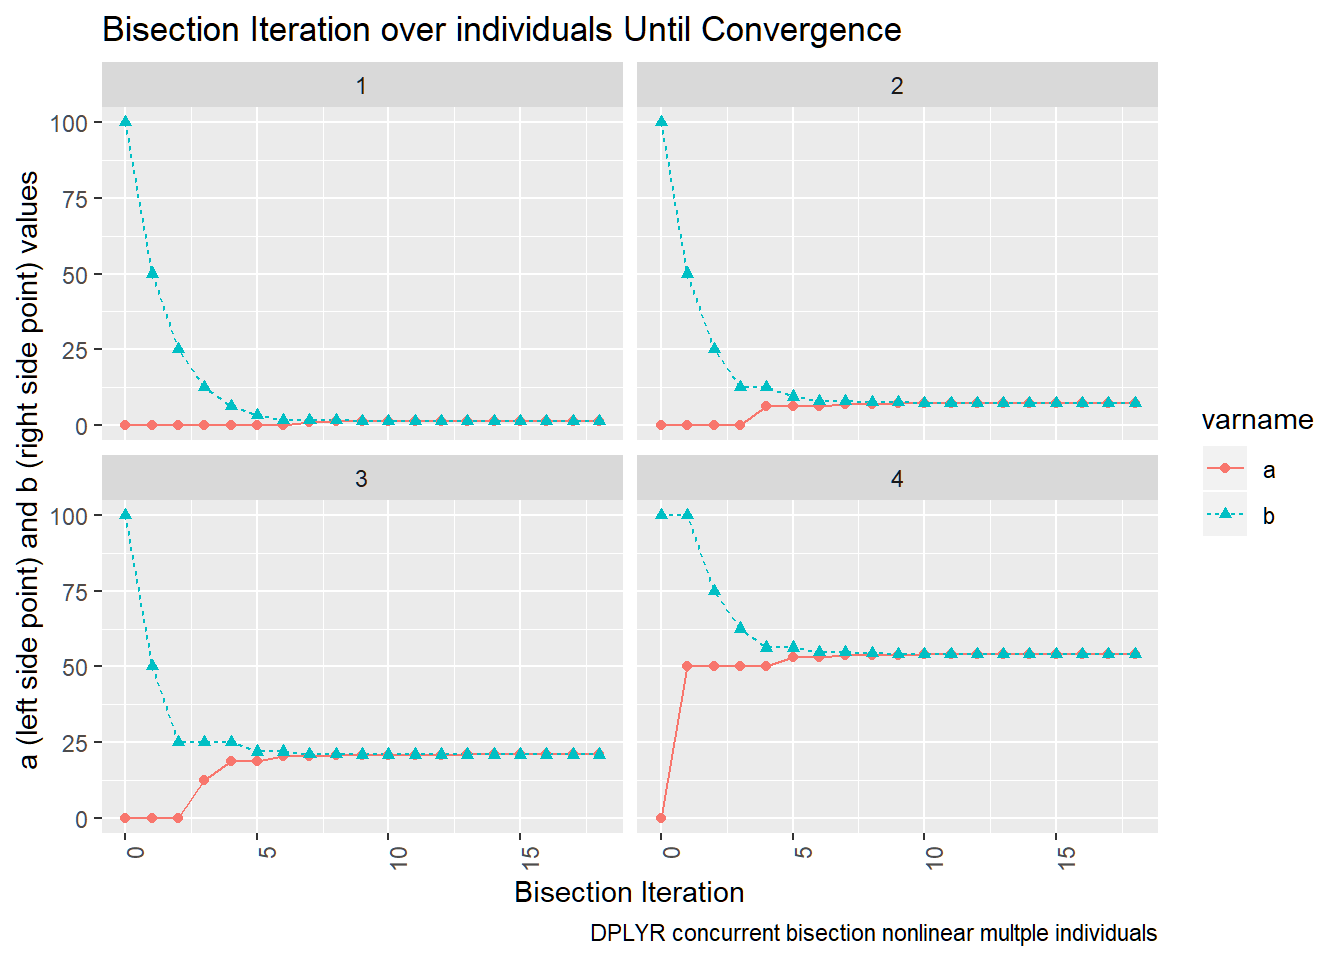
\includegraphics{fs_func_graph_eval_files/figure-latex/reshape solution for graphing-1.pdf}

\end{document}
